\documentclass{standalone}
\usepackage{tikz}
\usepackage{pgfplots}
\pgfplotsset{compat=1.18}
\usetikzlibrary{3d, angles, quotes}

\begin{document}
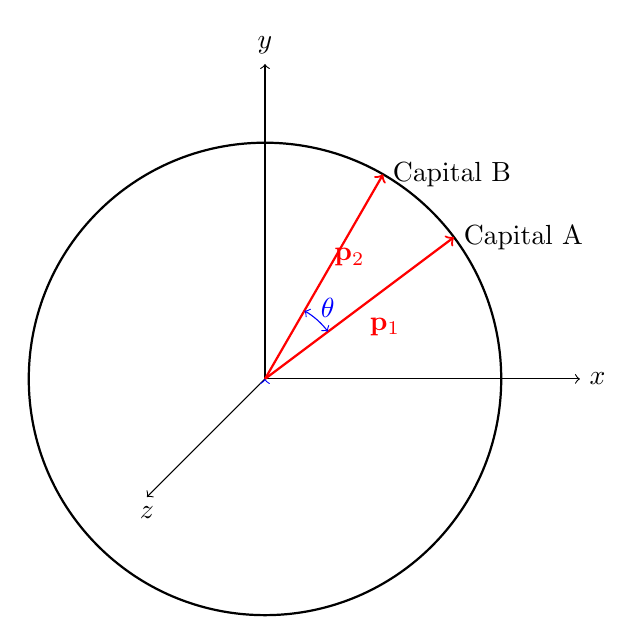
\begin{tikzpicture}
    % Draw the sphere (circle)
    \draw[thick] (0,0) circle (3cm);

    % Draw the 3D axes
    \draw[->] (0,0) -- (4,0) node[right] {$x$};
    \draw[->] (0,0) -- (0,4) node[above] {$y$};
    \draw[->] (0,0) -- (-1.5,-1.5) node[below] {$z$};

    % Define the points on the sphere surface
    \coordinate (P1) at (3*0.8,3*0.6);
    \coordinate (P2) at (3*0.5,3*0.866);
    
    % Draw vectors from the center to the points
    \draw[->, thick, red] (0,0) -- (P1) node[midway, below right] {$\mathbf{p}_1$};
    \draw[->, thick, red] (0,0) -- (P2) node[midway, above right] {$\mathbf{p}_2$};
    
    % Draw the angle between the vectors
    \draw[->, blue] (0,0) coordinate (O)
        pic["$\theta$", draw=blue, <->, angle eccentricity=1.2, angle radius=1cm]
        {angle=P1--O--P2};

    % Add some labels to the points
    \node at (P1) [right] {Capital A};
    \node at (P2) [right] {Capital B};
\end{tikzpicture}
\end{document}
